\documentclass[tikz,border=8pt]{standalone}
\usepackage[T1]{fontenc}
\usepackage{tikz}
\usetikzlibrary{arrows.meta,positioning}
\hyphenpenalty=10000
\exhyphenpenalty=10000

\definecolor{blueA}{RGB}{46,92,165}
\definecolor{greenA}{RGB}{45,132,92}
\definecolor{orangeA}{RGB}{190,115,35}
\definecolor{purpleA}{RGB}{115,80,160}
\definecolor{ink}{RGB}{45,50,60}

\tikzset{
  block/.style={
    rounded corners=3pt,
    draw=#1,
    very thick,
    fill=#1!8,
    text width=3.42cm,
    minimum height=2.25cm,
    align=center,
    inner sep=4.5pt,
    font=\sffamily\footnotesize
  },
  arrow/.style={-{Latex[length=2.5mm,width=1.8mm]}, line width=0.8pt, draw=ink},
  note/.style={
    rounded corners=2pt,
    draw=ink!35,
    fill=ink!4,
    text width=15.4cm,
    align=center,
    inner sep=4pt,
    font=\sffamily\footnotesize,
    text=ink
  },
}

\begin{document}
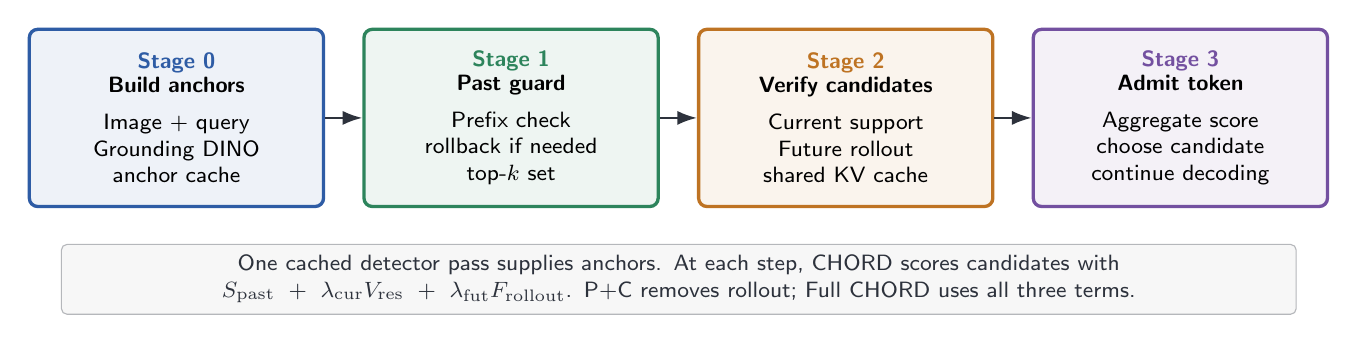
\begin{tikzpicture}[x=1cm,y=1cm]

\node[block=blueA] (s0) at (0,0) {
  {\sffamily\footnotesize\bfseries\textcolor{blueA}{Stage 0}}\\[-1pt]
  \textbf{Build anchors}\\[4pt]
  Image + query\\
  Grounding DINO\\
  anchor cache
};

\node[block=greenA] (s1) at (4.25,0) {
  {\sffamily\footnotesize\bfseries\textcolor{greenA}{Stage 1}}\\[-1pt]
  \textbf{Past guard}\\[4pt]
  Prefix check\\
  rollback if needed\\
  top-$k$ set
};

\node[block=orangeA] (s2) at (8.50,0) {
  {\sffamily\footnotesize\bfseries\textcolor{orangeA}{Stage 2}}\\[-1pt]
  \textbf{Verify candidates}\\[4pt]
  Current support\\
  Future rollout\\
  shared KV cache
};

\node[block=purpleA] (s3) at (12.75,0) {
  {\sffamily\footnotesize\bfseries\textcolor{purpleA}{Stage 3}}\\[-1pt]
  \textbf{Admit token}\\[4pt]
  Aggregate score\\
  choose candidate\\
  continue decoding
};

\draw[arrow] (s0.east) -- (s1.west);
\draw[arrow] (s1.east) -- (s2.west);
\draw[arrow] (s2.east) -- (s3.west);

\node[note] (formula) at (6.38,-2.05) {
  One cached detector pass supplies anchors. At each step, CHORD scores candidates with
  $S_{\mathrm{past}}+\lambda_{\mathrm{cur}}V_{\mathrm{res}}+\lambda_{\mathrm{fut}}F_{\mathrm{rollout}}$.
  P+C removes rollout; Full CHORD uses all three terms.
};

\end{tikzpicture}
\end{document}
